\part{CM10}
% Partie de Benoit Sluysmans a rajouter avant

Other undecidable problems :
\subsection{Malicious problem}
Input : A piece of code/program\\
Ouput : YES if malicious (virus)\\
The perfect anti-virus does not exist.

\subsection{Comparison between two programs}
Input : Two Matlab codes \texttt{M1.m} and \texttt{M2.m}\\
Ouput : YES if $M1(x) = M2(x)$ $\forall x$ (they compute the same function)\\
How do we prove the comparison problem is undecidable?
\paragraph{Proof} Suppose I want to check that $M$ halts on $x$. Then I create an instance of the comparison problem : 
\begin{itemize}
\item $M1(y) = M(x) \ \forall y$ (constant function)
\item $M2(y$) does not halt $\forall y$ (empty function, while true do 1)
\end{itemize}
If $M$ does not halt on $x$, then $M1(y) = M2(y) \ \forall y$. If M halts on $x$, then  $M1(y) \neq M2(y)$ for some $y$ (in fact, all of them but we don't even need it).
This is called a reduction of the halting problem to the comparison problem. It shows the halt problem is a particular case of the comparison problem, up to encoding. If we could solve the comparison problem algorithm, then we could solve the halt problem too.

\subsection{Arithmetic theorem problem}
Input : Logical formula of arithmetics ($\forall x, \exists y \cdots +, \times, \cdots$ with $x,y,\cdots \in \mathbb{N}$)\\
Ouput : YES if it is a theorem, i.e. it can be proved from basic rules of $=,\times$ and logic\\
For instance, $\forall x, \exists y : 2y = x$ is not a theorem but  $\exists x, \exists y : 2y = x$ is one.\\

Same question with $x,y,\cdots \in \mathbb{R}$ :  $\exists x : x^2+1=0$ is false but  $\forall x, \exists y : x^2+y=0$ is true. This problem is actually decidable. For instance, Sturm's theorem can find the number of distinct real roots of a polynomial located in an interval. Some questions about real numbers are actually easier than questions about integers.

\subsection{Matrix mortality problem}
Input : A finite set of $3\times3$ matrices with integral entries ($\in \mathbb{Z}^{3\times3}$)\\
Ouput : YES if there is a product of the matrices equal to $0$ (e.g. $M_1M_2M_1M_3M_1^2 = 0_{3\times3}$)

\subsection{Tiling problem (Berger, 1966)}
Input : A finite set of tetris-like shapes \\
Ouput : YES if you can tile the entire plan with copies of these shapes (e.g. Figure~\ref{Tiling})
\begin{figure}[!h]
                 \centering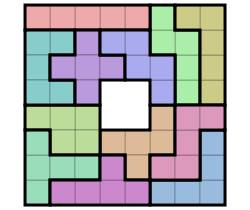
\includegraphics[width=0.3\textwidth]{pentomio.png}
         	\caption{Tiling problem}
        		\label{Tiling}
\end{figure}

\subsection{Diophantine equations (Matiyasevich, 1970)}
Input : A polynomial $P(x_1,\ldots, x_m)$ with coefficients in $\mathbb{Z}$ \\
Ouput : YES if $\exists x_1,\ldots, x_m \in \mathbb{Z} : P(x_1,\ldots, x_m) = 0$ \\


We can prove all that all these problems are undecidable by reduction from halting problem or other problems already proved undecidable.